\documentclass[a4paper,DIV=12,english]{scrartcl}
\usepackage[utf8]{inputenc}
\usepackage{fancyhdr}
\usepackage{bookmark}
\usepackage{graphicx}
\usepackage{hyperref}
\usepackage{xurl}
\usepackage[sorting=none, style=numeric-comp]{biblatex}
\addbibresource{ref.bib}
\usepackage{csquotes}
\usepackage[dvipsnames]{xcolor}
\usepackage[num]{isodate}
\usepackage{amsthm}
\usepackage{amssymb}
\usepackage{bbm}
\usepackage{amsmath}
\usepackage{tikz}
%\usepackage{pgfplots}
    %\usepgfplotslibrary{fillbetween}
\usepackage{svg}
\usepackage{braket}
\usepackage{caption}
\usepackage{subcaption}
\usepackage{placeins}
%\setlength\parindent{0pt}
\usepackage{wrapfig}
\usepackage{float}


% Fakesection
\newcommand{\fakesection}[1]{%
    \par\refstepcounter{section}                                        % Increase section counter
    \sectionmark{#1}                                                    % Add section mark (header)
    \addcontentsline{toc}{section}{\protect\numberline{\thesection}#1}  % Add section to ToC
    % Add more content here, if needed.
} 

\renewcommand{\footrulewidth}{0.5pt}
\pagestyle{fancy}
\fancyhf{}
\fancyhead[L]{\leftmark}
\fancyhead[R]{}

\fancyfoot[C]{Computational Physics: Temperature of Earth}
\fancyfoot[R]{\thepage}

\title{Computational Physics: Temperature of Earth Project Report}
\author{Stockholm University, Spring Term 2024 \\Max Maschke}
\date{Apr 04 2024}


\begin{document}
\maketitle


\tableofcontents
\newpage


\newpage
\section{Introduction}
In this report, a simple energy balance model of Earth's atmosphere is presented, implemented and analysed. It is part of the coursework for the computational physics class held at Stockholm University in 2024.

\section{Energy Balance Models}
Energy balance models (EBMs) arguably represent the simplest class of climate models. They model the temperature of the Earth system using simple energy flux considerations only~\cite{ebcms}. 

The simplest realisation of such a system is what's sometimes referred to as the zero-dimensional energy balance model: the temperature is calculated using the Stefan-Boltzmann law
\begin{equation}
    \frac{P}{A} = \sigma T^4,\quad \sigma = \frac{2\pi^5 k_\text{B}^4}{15 h^3c^2}\approx 5.69 \frac{\text{W}}{\text{m}^2\text{K}^4},
\end{equation}
assuming a steady state in which the Earth emits precisely the incoming flux at all times. Such a model predicts a surface temperature of -21°~C, which is much too low.

The most important property of the Earth system that is neglected in the above model is the planet's atmosphere. Absorption in the atmosphere traps a portion of the incoming flux, which is known as the greenhouse effect.

In this analysis an energy balance model for a zero-dimensional planet with a one-dimensional atmosphere that is extended in the $z$-direction is studied, thus neglecting any convective effects and the water cycle. The incoming light is restricted to a single wavelength in the visible part of the spectrum and any thermally emitted light is in turn restricted to a single IR wavelength. This implies that there is only one absorption cross-section $\sigma_i,~i=\text{IR, V}$, for both parts of the spectrum.

To make the model numerically tractable, the atmosphere is divided into $n$ discrete layers of height $dh$. In any of these layers $j$, the energy balance is given by
\begin{equation}
    E_j = A_j,
\end{equation}
that is emission must equal absorption. All radiation incoming from neighbouring layers that is not transmitted is absorbed, so 
\begin{equation}\label{emission}
    E_j = A_j = \left(\frac{E_{j-1} + E_{j+1}}{2} + T_{j-1}^{\text{out}} + T_{j+1}^{\text{in, IR}}\right)\left(1 - \text{e}^{-\sigma_\text{IR}\rho_j dh}\right) + T_{j+1}^{\text{in, V}}\left(1 - \text{e}^{-\sigma_\text{V}\rho_j dh}\right).
\end{equation}
The equations for the different transmission measures are omitted here for brevity and can be found in the course material. The lowest layer is assumed to be a black body, which is a first order approximation for the Earth's surface:
\begin{equation}
    E_0 = A_0 = \frac{1}{2}E_1 + T_{j+1}^{\text{in, IR}} + T_{j+1}^{\text{in, V}}
\end{equation}

It can be immediately seen that absorption depends on the density of the atmosphere at a given height $h_j = j\cdot dh$. From the ideal gas law
\begin{equation}\label{density}
    \frac{M}{V} = \rho = \frac{Pm}{k_\text{B}T}
\end{equation} 
where $m$ is the molecular mass of air, and the hydrostatic condition considering the height-variation of the gravitational acceleration $g$
\begin{equation}
    \frac{\text{d}P}{\text{d}h} = -\rho \cdot g(h),
\end{equation}
we find
\begin{equation}\label{ODE}
    \frac{\text{d}P}{\text{d}h} = -\frac{Pm}{k_\text{B}T} \cdot g(h).
\end{equation}
Assuming $T=\text{const.}$, this differential equation can be solved iteratively given a starting value for $P$. The density is then directly calculated from $P$ using equation~\eqref{density}.

\section{Numerical Formulation}
\subsection{Density calculation}
Since the density in principle only has to be calculated once for all the other calculations, a more expensive but more accurate solver than a simple Euler method
\begin{equation}
    P_{i+1} = P_i + \frac{\text{d}P}{\text{d}h}(h_{i})\cdot \text{d}h
\end{equation}
can be used for increased accuracy. We chose to apply a three-step Adams–Bashforth method:
\begin{equation}
    P_{i+1} = P_i + \left(\frac{23}{12}\frac{\text{d}P}{\text{d}h}(h_{i}) - \frac{16}{12}\frac{\text{d}P}{\text{d}h}(h_{i-1}) + \frac{5}{12}\frac{\text{d}P}{\text{d}h}(h_{i-2}) \right)\cdot\text{d}h
\end{equation}
Note that the first two steps have to be taken using Euler steps or similar. This method has error of order $O(dh^3)$ instead of the Euler method's $O(dh)$~\cite{wiki_adams_bashforth}.

\subsection{Iterative EBM solution}
The set of equations describing the model, namely \eqref{emission} etc., are coupled and must thus be solved consistently. One approach to this is to initialise $T_{n}^{\text{in, V}} = 1$ and then propagate the quantities $T^{\text{in, V}}$, $T^{\text{in, IR}}$ and $E$ downwards. Subsequently, starting from $E_0$, $T^{\text{out}}$ can be propagated upwards. This procedure can be repeated as many times as required until a steady solution is found. 

This scheme is advantageous since it is very quick, requiring only $2n \cdot n_\text{sweep}$ iterations where $n_\text{sweep}$ is the number of full sweeps done. However, some boundary conditions that we might want to impose on the model are not explicitly enforced. For example, the outgoing flux $E_n/2 + T^{\text{out}}_n$ should be equal to the incoming visible flux, but the iteration does not guarantee this so it must be checked.

\subsection{Direct EBM solution}
Another approach is to realise that the equations describing the model constitute a linear system $Ax = b$ with $4n + 4$ unknowns if we include an $n+1$-th layer representing space where the density has dropped to zero. If $A$ is non-singular, the system has a unique solution. To ensure $A$ has full rank, the following additional boundary conditions have to be imposed:
\begin{align}
    T_{n+1}^{\text{in, V}} &= 1 \nonumber \\
    T_{n+1}^{\text{in, IR}} &= 0 \nonumber \\
    T_{0}^{\text{out}} &= E_0 \\
    T_{n+1}^{\text{out}} &= 1 \nonumber \\
    E_{n+1} &= 0 \nonumber
\end{align}
In English, these mean that, a), the incoming visible flux is normalised, b), no IR flux is incoming from the sun, c), the ground emits as a black body, d), the outgoing IR radiation must be equal in energy flux to the incoming visible flux and e), space does not absorb or emit.

From here, the methods discussed last week can be applied to solve the linear system directly. The advantage is that the solution will obey the boundary conditions exactly. However, calculating the $LU$-decomposition for a system of size $4n+4 \times 4n+4$ becomes costly quite quickly as $n$ is increased. As will be seen later, this method is thus not very efficient. Another problem with the interpretability of the directly obtained solution was also encountered later, namely that $E_0$, from which the temperature is obtained, came out to be negative, which is unphysical.

\section{Implementation and Numerics}
The calculation of the density and the solving of the EBM are implemented in Python. The code is enclosed with this report and also available at~\cite{github}. To speed up the iteration which would otherwise be performed in the interpreter, the code is just-in-time compiled using \texttt{Numba}~\cite{numba}. The LSE is solved using \texttt{Numpy}'s \texttt{linalg.solve} function~\cite{harris2020array}, which internally calls on \texttt{LAPACK}~\cite{laug} to compute the $LU$-decomposition.

Values of the important physical constants and measurements such as the sea level pressure are taken from~\cite{Wolfram}, cf. the head of \texttt{physics.py}~\cite{github}. The cut-off for the atmosphere is chosen to be $h_\text{max}=100\,\text{km}$, which implies that if, e.g., 10000 layers are used, $dh=10\,\text{m}$. The Earth's albedo is fixed at 0.33 and a solar flux of $344 \text{W}/\text{m}^2$ is used. Due to limited time, the influence of the mean surface reflectivity could not be implemented nor studied. The absorption in the visible bands was fixed at $\alpha_\text{V}=5\cdot 10^{-5}/\text{m}$
\subsection{Performance}
\begin{figure}
    \centering
    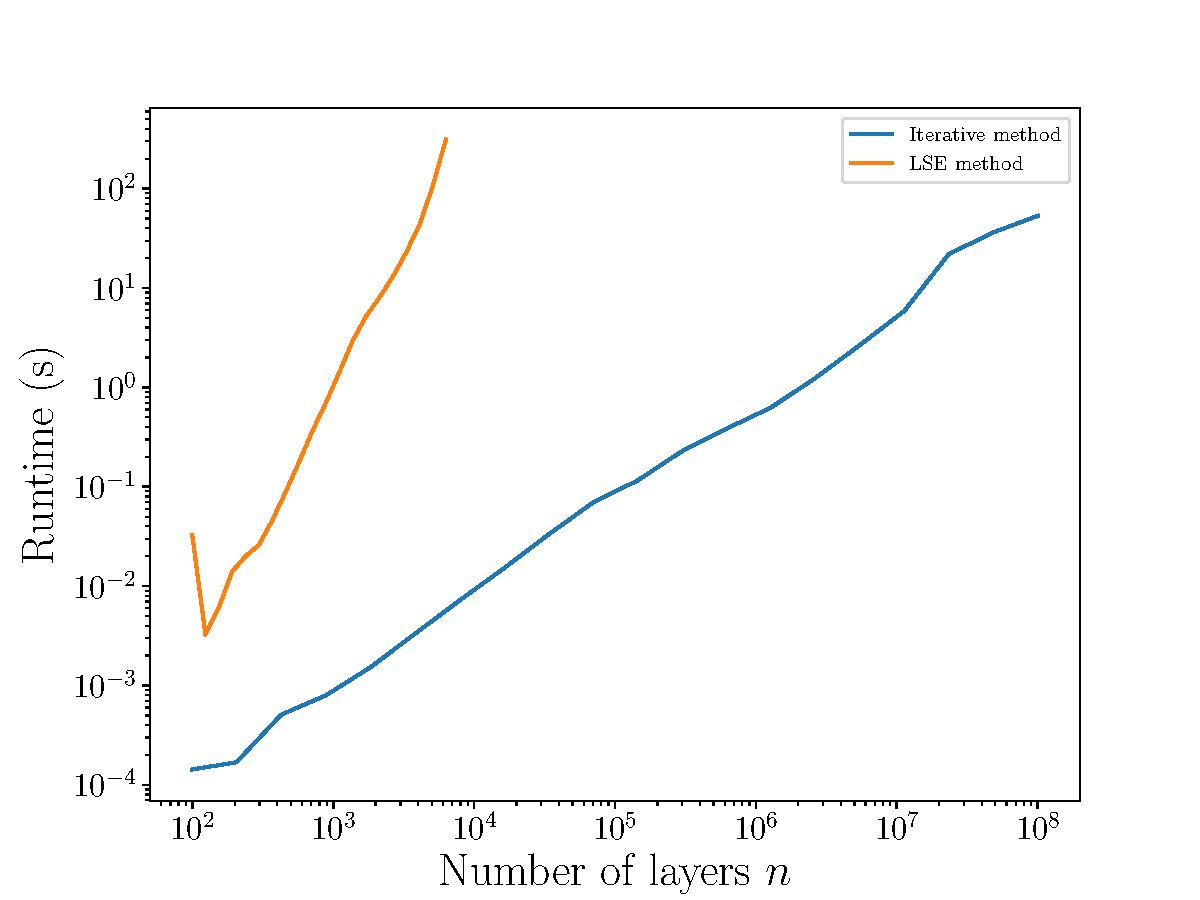
\includegraphics[width=0.5\textwidth]{../plots/performance.pdf}
    \caption{Measured runtimes of solving the EBM using the iterative and the LSE based approaches. The iteration, which used 15 full sweeps, outperforms the LSE solver by orders of magnitude and thus allows the study of much finer layers. Both curves have different slopes in the logarithmic plot, indicating that the iteration is $O(n\cdot n_\text{sweep})=O(n)$ while the LSE solver is $O\left((4n+4)^3\right)$.}
    \label{fig:performance}
\end{figure}
The measured runtimes of solving the EBM using both approaches is shown in figure~\ref{fig:performance}. It can be seen that the iteration, which used 15 full sweeps, outperforms the LSE solver by orders of magnitude and thus allows the study of much finer layers. It can also be seen that the iteration is $O(n\cdot n_\text{sweep})=O(n)$ while the LSE solver is $O\left((4n+4)^3\right)$.

\subsection{Numerics}
More important than the performance of any numerical method are its stability and convergence. To investigate this for both methods, their behaviour as the main numerical parameter $n$ is tuned must be observed.
\begin{figure}
    \centering
    \begin{subfigure}{0.49\textwidth}\
        \centering
        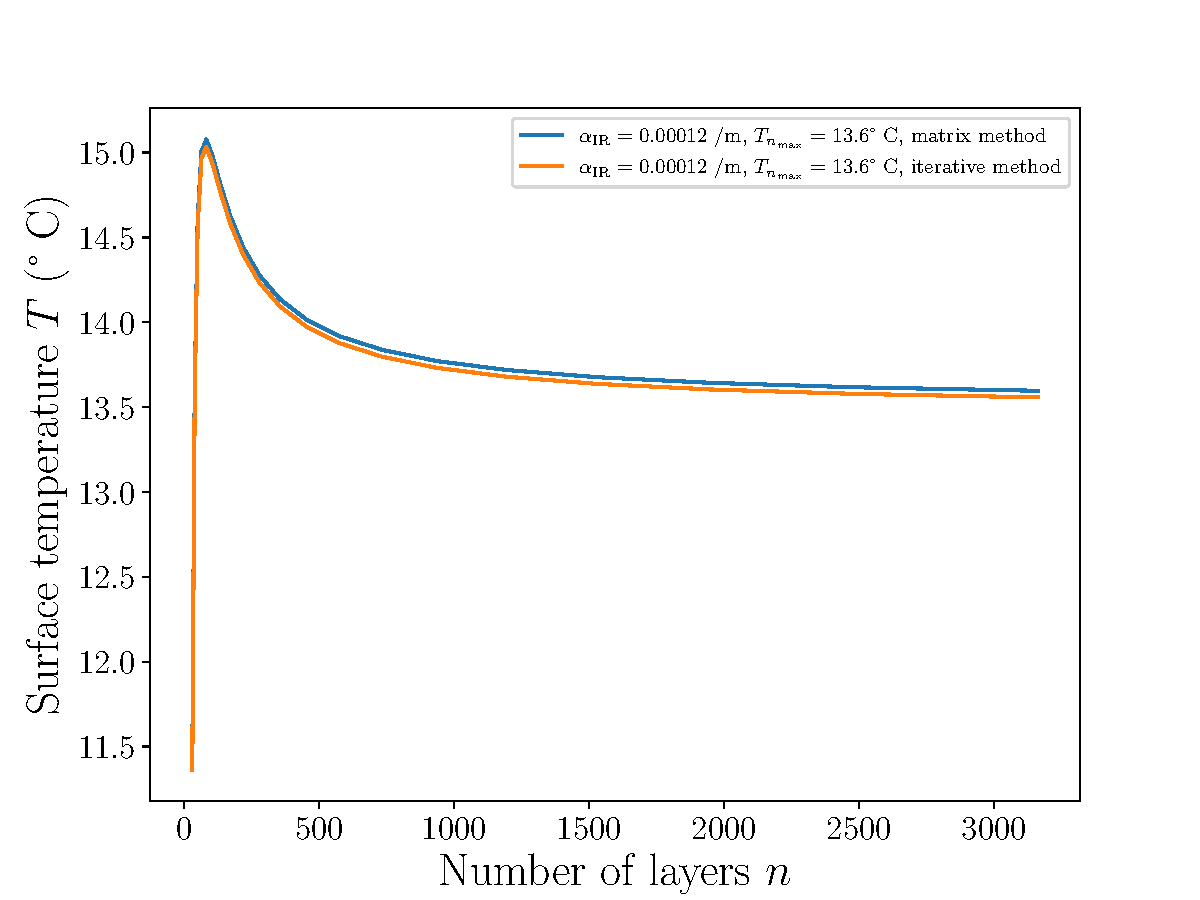
\includegraphics[width=\textwidth]{../plots/temp_comp/full_N_comp.pdf}
        \caption{Comparison of the predicted surface temperature for varying $n$ for both methods, using $\alpha_{\text{IR}}=1.2\cdot 10^{-4}/\text{m}$. Both methods converge and agree up to the first decimal.}
        \label{subfig:N_comp}        
    \end{subfigure}
    \begin{subfigure}{0.49\textwidth}\
        \centering
        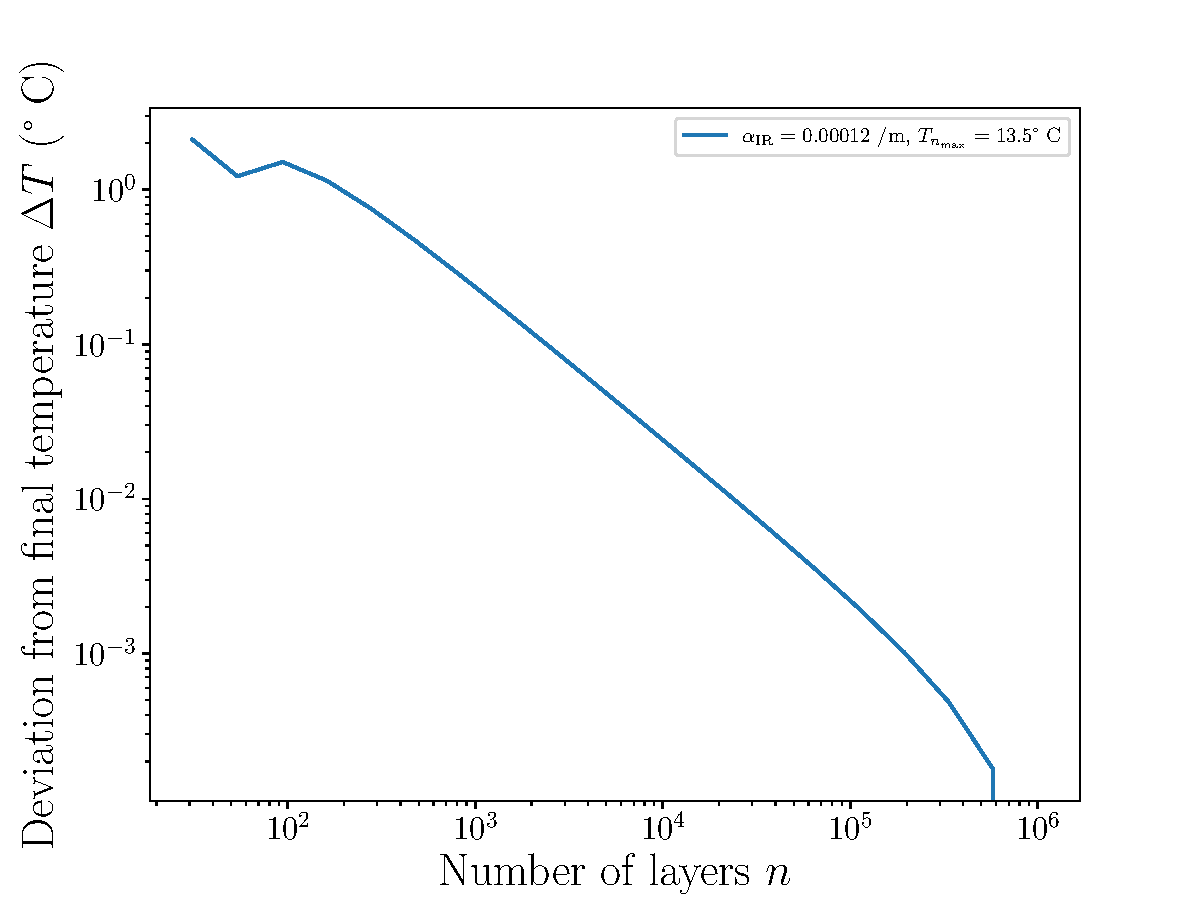
\includegraphics[width=\textwidth]{../plots/temp_full_it/full_N.pdf}
        \caption{Convergence towards the final value for the iterative method using $\alpha_{\text{IR}}=1.2\cdot 10^{-4}/\text{m}$. To achieve three decimals of numerical accuracy, $10^5$ layers are needed.}
        \label{subfig:N_it}        
    \end{subfigure}    
    \caption{Numerics of increasing $n$ for both approaches. Both methods are seen to be stable for increasing $n$ in the parameter ranges studied.}
    \label{fig:N}
\end{figure}

Figure~\ref{fig:N} shows how both models respond to increasing $n$. Not only do both of them show numerical convergence, they also agree up to the first decimal for $n=3000$ layers. Much finer layers are numerically intractable for the LSE method, but with the iterative method, we can go up to $n=10^8$. The additional precision gained by this is sure to be offset by systematic sources of error in the choice of physical parameters and approximations of the model, so such a high number of discretisations is not needed in practice, which is why $n=105$ was used consistently later on.
\begin{figure}
    \centering
    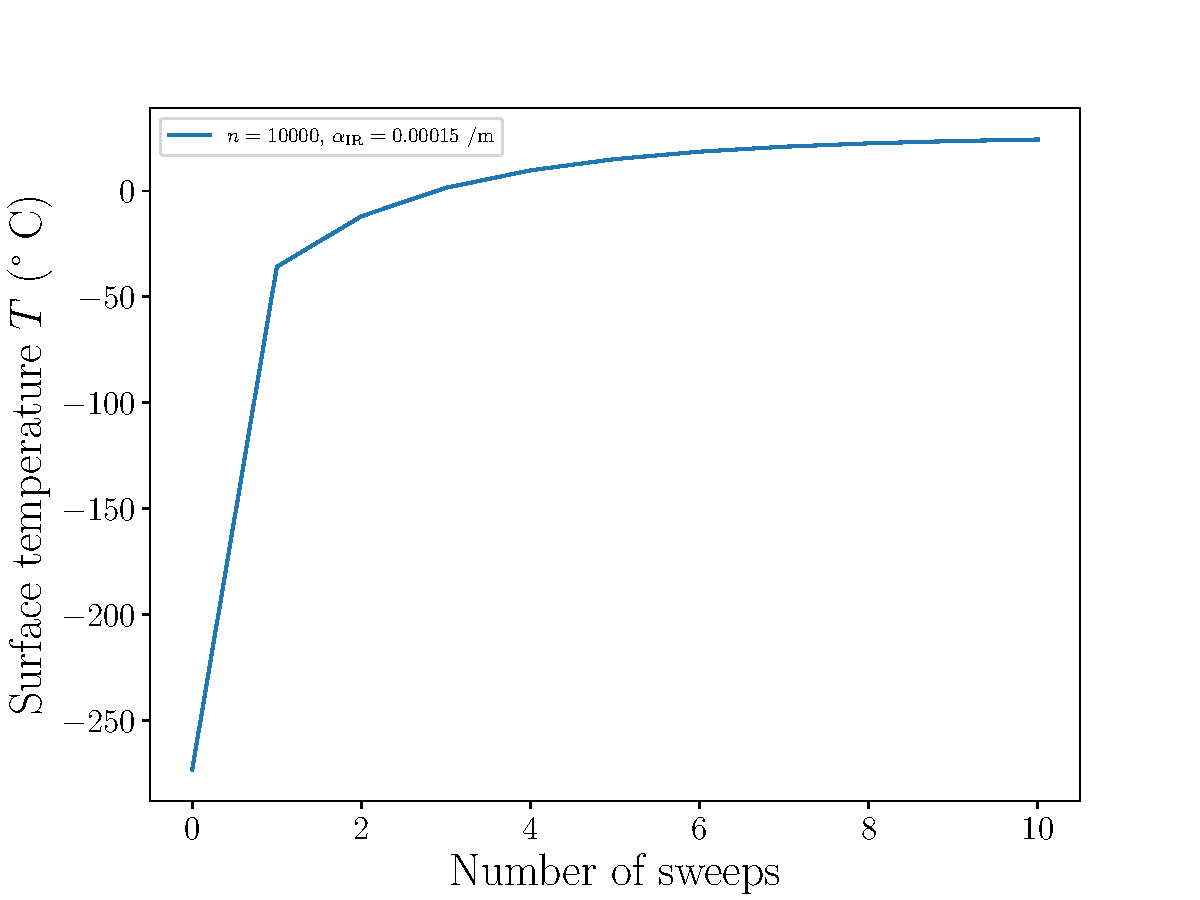
\includegraphics[width=0.65\textwidth]{../plots/temp_full_it/full_sweeps.pdf}
    \caption{Numerics of increasing the number of sweeps for the iterative method, using $\alpha_{\text{IR}}=1.2\cdot 10^{-4}/\text{m}$ and $10^5$ layers. To achieve two decimals of convergence, 15 sweeps are needed.}
    \label{fig:sweeps}
\end{figure}

For the iterative method, there is another numerical parameter, namely the number of sweeps $n_\text{sweeps}$. Figure~\ref{fig:sweeps} shows the numerical convergence of increasing this quantity. It can be clearly seen that at least a handful of sweeps are required for the temperature to settle. We estimate that the two decimals of convergence given by using 15 sweeps is enough precision for the rest of this analysis and thus used this amount henceforth.

It is important to note that the iteration did not exactly achieve $T_{n+1}^{\text{in, V}} = T_{n+1}^{\text{out}} = 1$. The latter fluctuated in a typical range of 0.5 to 2. Unfortunately, there was not enough time left to investigate this further, but it is surprising given that the LSE and the iteration agree in their predictions for surface temperature and the LSE enforces this condition strictly.

\section{Physical Predictions}
In this section, the physical predictions of the model are to be discussed.

\subsection{Density}
Before the temperatures are looked at, the validity of the ODE solution giving the density is to be confirmed. It has to be reiterated here that the density curve depends on a guess of temperature that is assumed to be constant while the density is calculated. This has only a slight influence on the results, though, as long as this guess for $T$ is kept in a reasonable range. We used $T=15\text{° C}$ henceforth to ensure that the density at $h=0$ which is derived from the pressure at sea level is as close to the literature value for sea level density as possible, see figure~\ref{fig:density}.
\begin{figure}
    \centering
    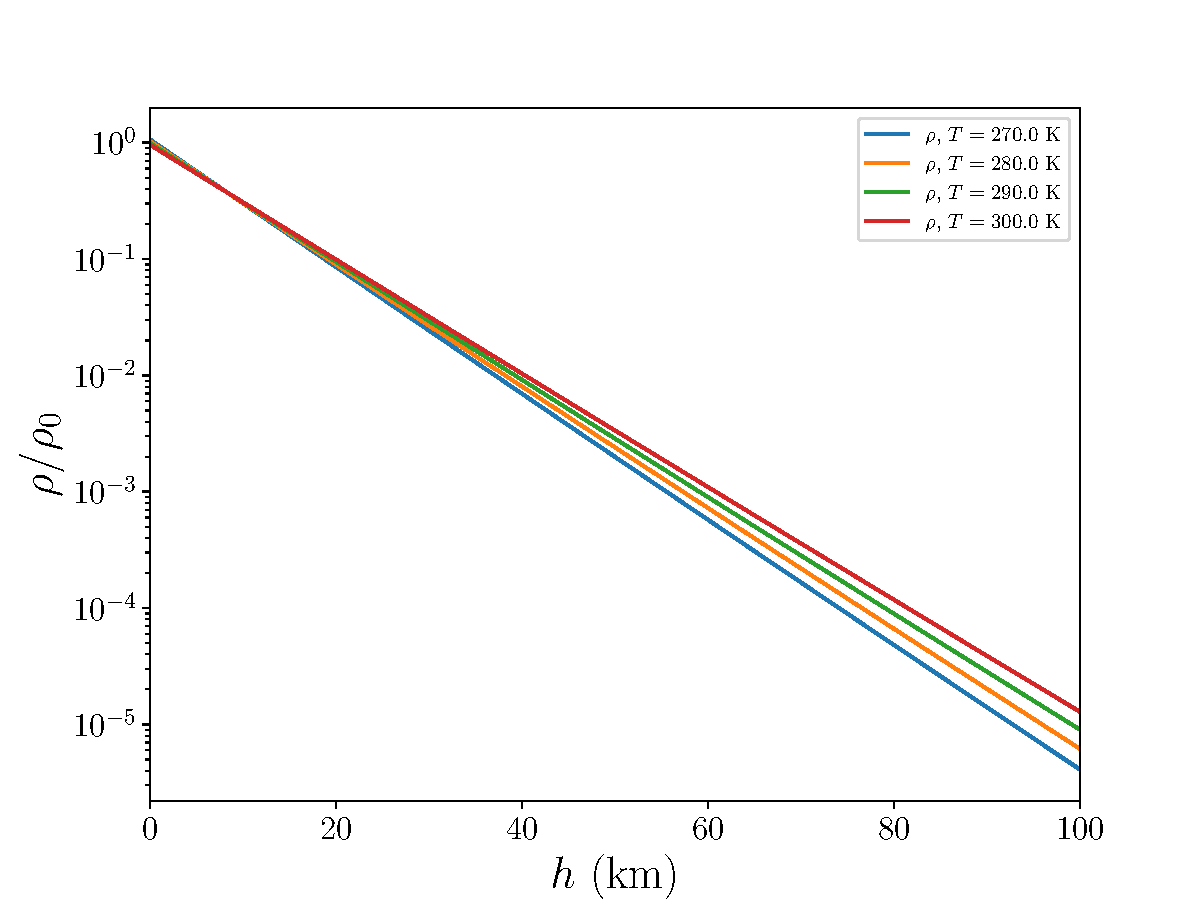
\includegraphics[width=0.65\textwidth]{../plots/density/density.pdf}
    \caption{Density profile of the atmosphere obtained from numerically solving equation~\eqref{ODE} for different temperature guesses. The choice of temperature more strongly affects the densities at higher heights than at sea level.}
    \label{fig:density}
\end{figure}

The approximately linear drop on the lin-log plot implies that the drop in density is roughly exponential, which is what our first order expectation would be considering the barometric formula known from introductory physics classes.

\subsection{Sea level temperature predictions}
The predicted sea level temperature of the model strongly depends on the absorption in the IR bands, parametrised by 
\begin{equation}
    \alpha_{\text{IR}} = \sigma_\text{IR} \cdot \rho_0
\end{equation}
where $\rho_0$ is the sea level density. Given more time, it would have been prudent to determine a reasonable range for this parameter from known concentrations of greenhouse gases in the atmosphere. Instead, we are forced to limit our analysis to varying $\alpha_{\text{IR}}$ with the goal of predicting the average temperature of Earth, $T_\text{E}\approx 15\text{° C}$.

The predicted sea level temperature for a large range of values of $\alpha_{\text{IR}}$ is shown in figure~\ref{subfig:alpha_comp} for both the iterative and the LSE method, using $n=3000$ layers. We see that at low $\alpha_{\text{IR}}$, they are in excellent agreement, however, beyond a certain point, the LSE method breaks down. This is because the predicted surface emission becomes negative, which is unphysical. The reason for this could not be definitely determined but may have to do with the condition of the matrix as $\alpha_{\text{IR}}$ is increased. By design, the iterative method does not depend on the rank of the coefficient matrix $A$, so it does not show this problem. For the iterative method, the plot is repeated in figure~\ref{subfig:alpha_full} for a higher $n$ of $10^5$, showing minimal differences except for very large $\alpha_{\text{IR}}$.

Physically, we see that our model shows the greenhouse effect as desired. In the absence of IR-absorbing gases, i.e.\ as $\alpha_{\text{IR}}\longrightarrow 0$, the predicted temperature is quite cold and close to that of the zero-dimensional EBM. Note that it is slightly lower than the 21° C quoted above since visible absorption is present in the model which reduces the flux that reaches the surface.

Conversely, as $\alpha_{\text{IR}}$ is increased, the temperature rises and, at very high and possibly unphysical $\alpha_{\text{IR}}$, plateaus. Figure~\ref{subfig:alpha_log} shows that for an $\alpha_{\text{IR}}$ of ca.\ $1.2\cdot 10^{-4}/\text{m}$, the predicted temperature is approximately 15° C which is the roughly expected real value.

\begin{figure}
    \centering
    \begin{subfigure}{0.49\textwidth}
        \centering
        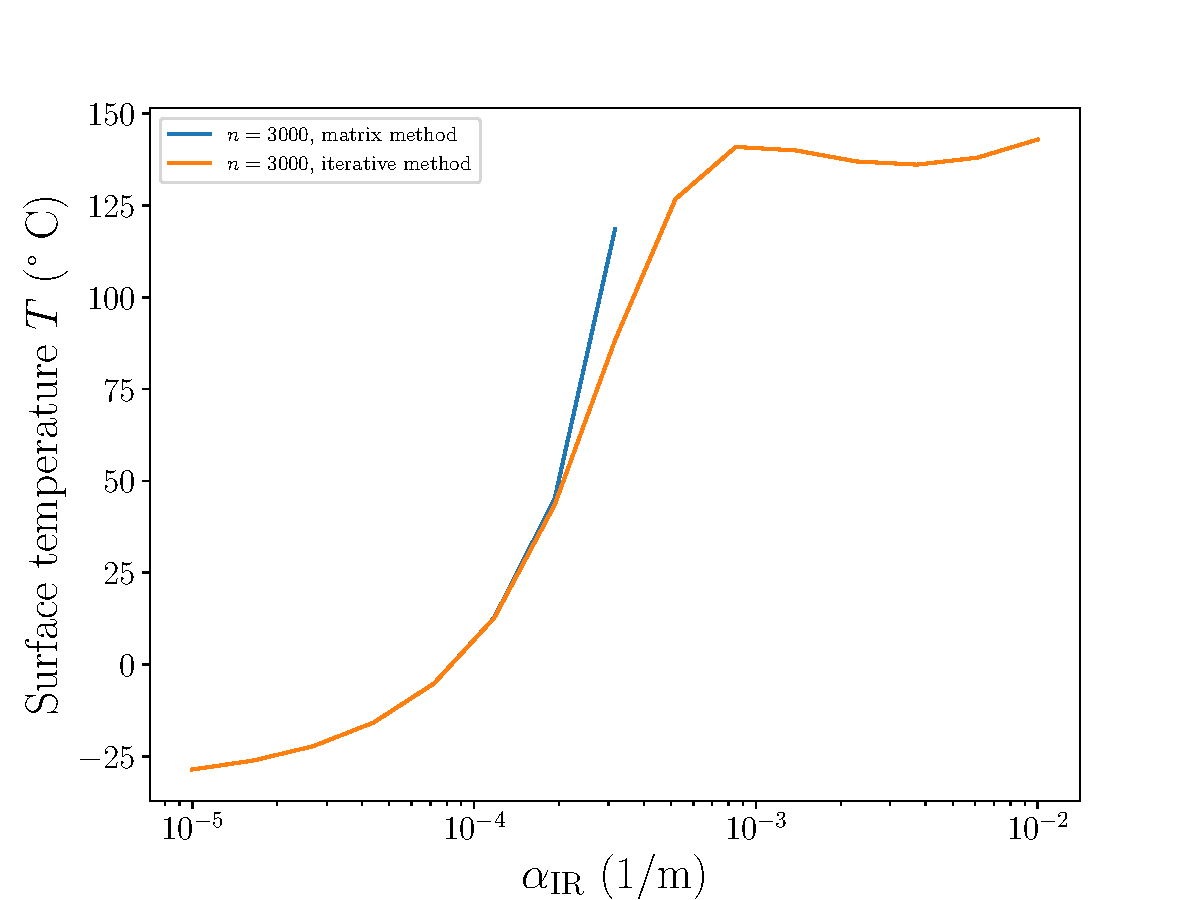
\includegraphics[width=\textwidth]{../plots/temp_comp/full_alpha_comp.pdf}
        \caption{Predicted sea level temperature for a large range of values of $\alpha_{\text{IR}}$, both methods, $n=3000$. For large $\alpha_{\text{IR}}$, the LSE method breaks down.}
        \label{subfig:alpha_comp}
    \end{subfigure}\begin{subfigure}{0.49\textwidth}
        \centering
        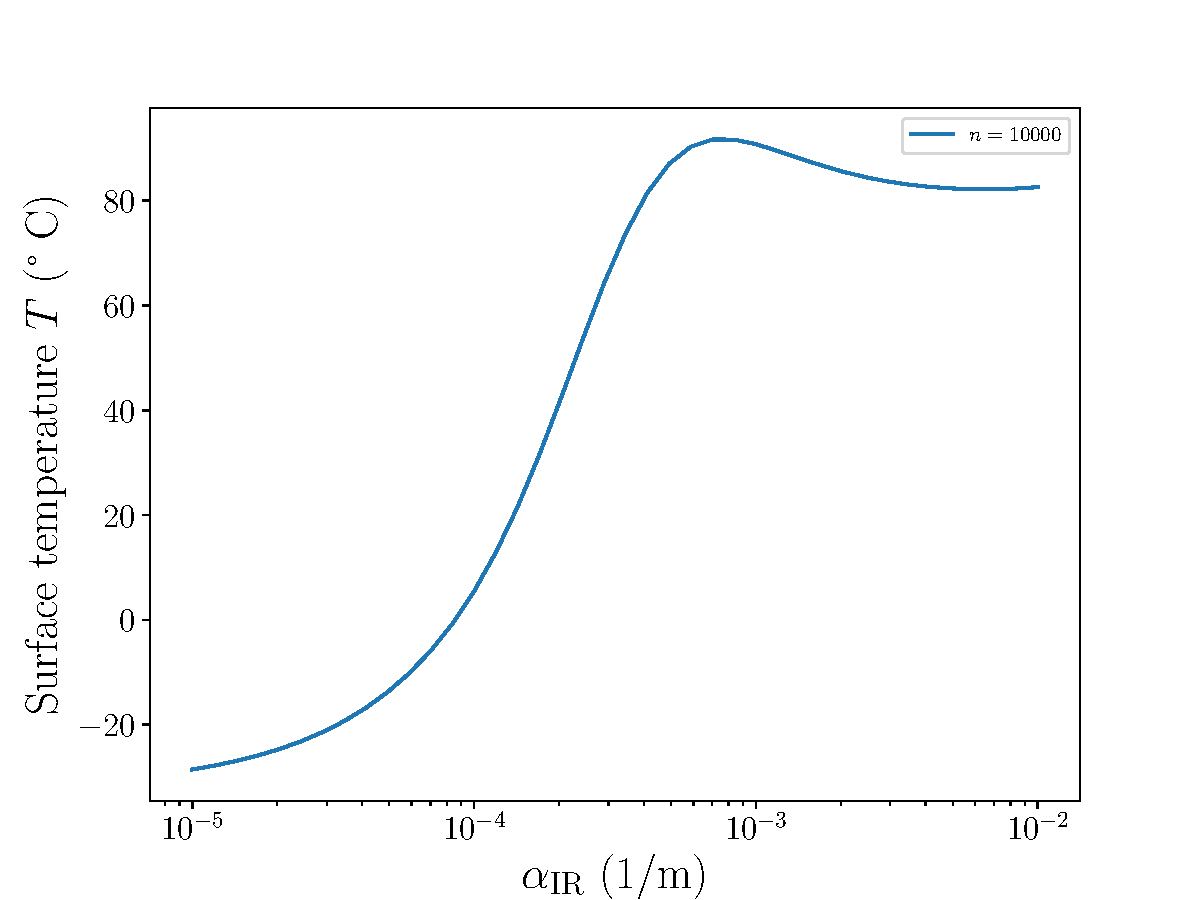
\includegraphics[width=\textwidth]{../plots/temp_full_it/full_alpha.pdf}
        \caption{Predicted sea level temperature for a large range of values of $\alpha_{\text{IR}}$, iterative method, $n=10^5$. The iterative method is stable for all $\alpha_{\text{IR}}$.}
        \label{subfig:alpha_full}
    \end{subfigure}\\
    \begin{subfigure}{0.49\textwidth}
        \centering
        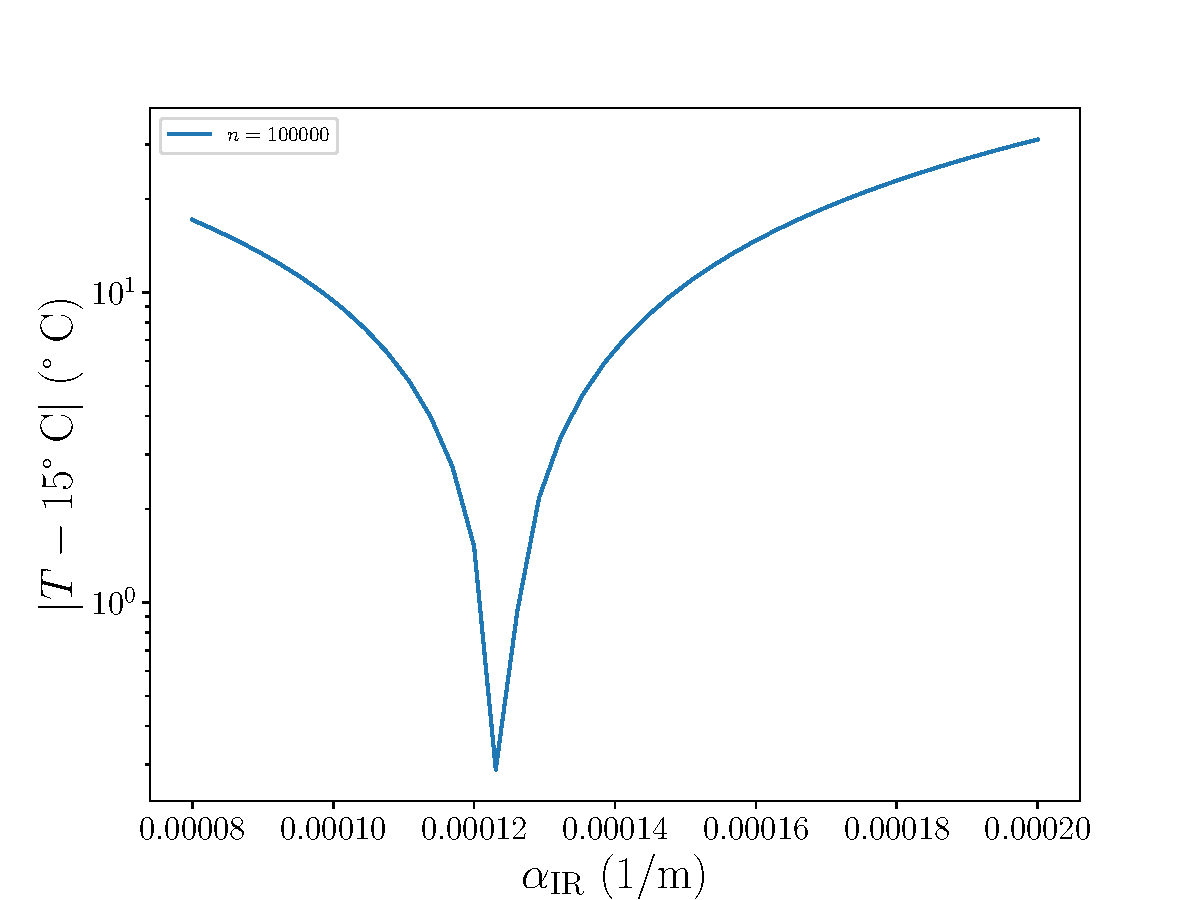
\includegraphics[width=\textwidth]{../plots/temp_full_it/full_alpha_log.pdf}
        \caption{Predicted sea level temperature for a narrow range of values of $\alpha_{\text{IR}}$, iterative method, $n=10^5$. An $\alpha_{\text{IR}}$ of ca. $1.2\cdot 10^{-4}/\text{m}$ reproduces the expected value.}
        \label{subfig:alpha_log}
    \end{subfigure}
    \caption{Sea level temperature predictions of the EBM for varying $\alpha_{\text{IR}}$.}
    \label{fig:alpha}
\end{figure}

\FloatBarrier
\subsection{Atmospheric temperature}
\begin{figure}[h]
    \centering
    \begin{subfigure}{0.49\textwidth}
        \centering
        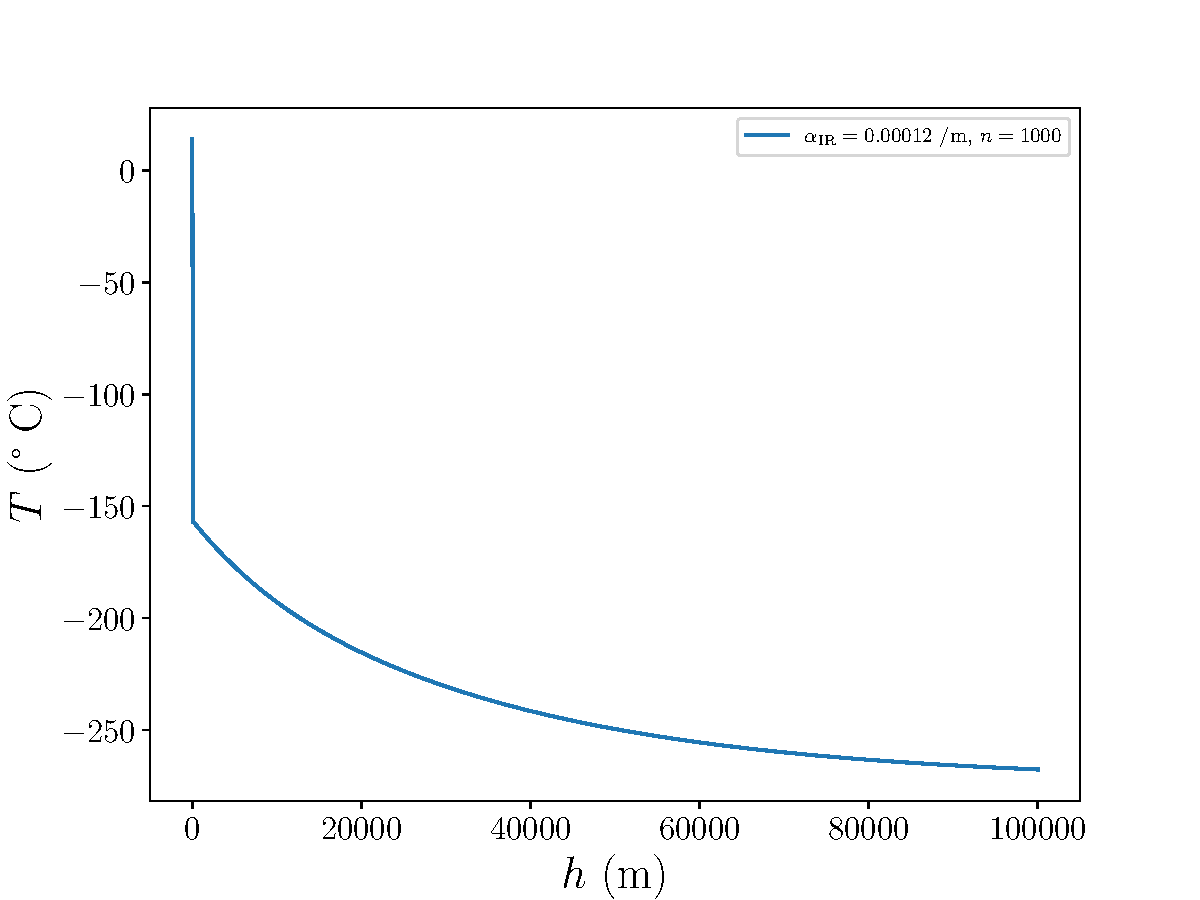
\includegraphics[width=\textwidth]{../plots/T_height/T_height_mat.pdf}
        \caption{LSE}
        \label{subfig:height_mat}
    \end{subfigure}
    \begin{subfigure}{0.49\textwidth}
        \centering
        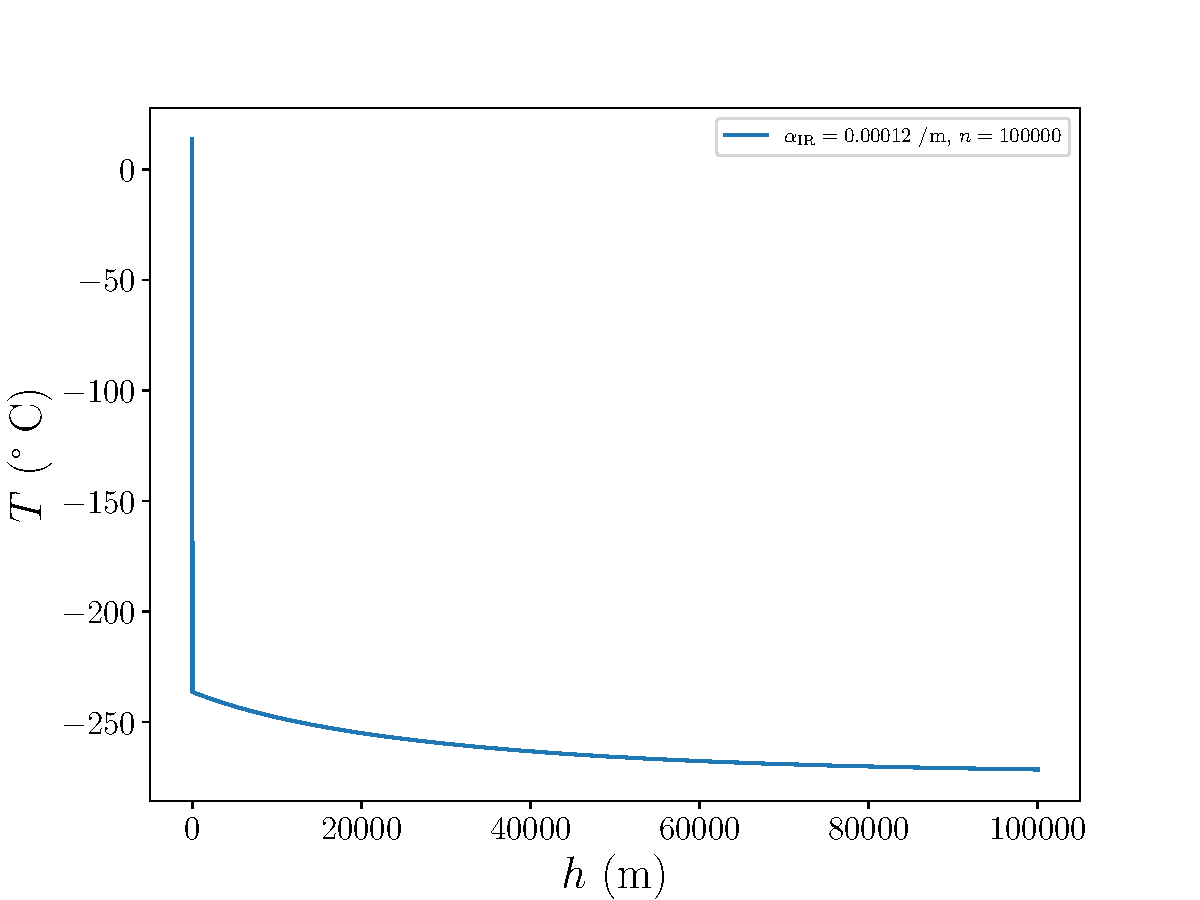
\includegraphics[width=\textwidth]{../plots/T_height/T_height_it.pdf}
        \caption{Iteration}
        \label{subfig:height_it}
    \end{subfigure}
    \caption{Temperature profile of the atmosphere predicted using the EBM.}
    \label{fig:height}
\end{figure}
As a last step, we want to see how the temperature of the atmosphere varies with height. This is shown in figure~\ref{fig:height}. It appears that while the ground layer is at high temperature, the atmosphere it is supposed to be in thermal equilibrium with has much too low temperature even in the first layer above the ground. This could either be because the way the temperatures were calculated using the Stefan-Boltzmann law is wrong for the atmosphere, or there is a previously undiscovered mistake somewhere else in the model. The latter would be discouraging because it would mean that the model does not make physically meaningful predictions but is instead just fitted such that the surface temperature matches expectation.

Due to a lack of time, we can sadly not investigate this further.

\section{Conclusion}
In this report, we presented our implementation of the EBM described and discuss its numerics and physical predictions. Unfortunately, in the last step, a large problem emerged that we could not solve in time, which makes any interpretation of the results discussed before dubious.

\newpage
\FloatBarrier
\fakesection{References}
\printbibliography


\end{document}
